\documentclass[12pt]{article}
	\addtolength{\oddsidemargin}{-.4in}
	\addtolength{\evensidemargin}{-.4in}
	\addtolength{\textwidth}{0.8in}
	\addtolength{\topmargin}{-0.8in}
	\addtolength{\textheight}{1.4in}
\usepackage{float}
\usepackage[margin=2.5cm]{geometry}
\usepackage{graphicx}
\usepackage[english]{babel}
%\usepackage{textgreek}
\usepackage{url}
\usepackage{amssymb}
\usepackage{epsfig}
\usepackage{bbm}
\usepackage{bbold}
\usepackage{graphicx}
\usepackage{amsmath}
\def\jddot#1{\stackrel{\bigdot\bigdot}{#1}}
\def\L{\mathcal L}
\def\e{\varepsilon}
\def\simlt{\stackrel{<}{{}_\sim}}
\def\simgt{\stackrel{>}{{}_\sim}}
\def\be{\begin{equation}}
\def\ee{\end{equation}}
\newcommand{\nucl}[3]{
\ensuremath{
\phantom{\ensuremath{^{#1}_{#2}}}
\llap{\ensuremath{^{#1}}}
\llap{\ensuremath{_{\rule{0pt}{.75em}#2}}}
\mbox{#3}
}
}





%\bibpunct{(}{)}{;}{a}{ }{,}
\begin{document}
\bibliographystyle{IEEEtran}

\title{Literature Review}
\author{Samuel Murphy-Sugrue\\}
 %School of Physics and Astronomy\\
 %University of Southampton\\
 %Southampton SO17 1BJ
 %Supervised by Pasquale Di Bari}

\maketitle
\clearpage
\tableofcontents
\clearpage


\section{Introduction}
\paragraph{•}
Talk about the main aims of the project and motivation for it. EG understanding probe theory in magnetised plasmas, essential for fusion

Probes as well as other diagnostics are used at the edge of tokamaks and other fusion devices to make measurements of the plasma conditions. Divertors are required at the edge of the tokamak in order to remove helium ash produced from fusion and other impurities that have entered the plasma from the edge of the vessel. The future success of fusion depends on the development of more advanced divertor schemes that can take out the plasma impurities and withstand the high heat fluxes long enough to make the machine economically viable. The development of more sophisticated divertors requires an improved understanding of plasma transport inside the tokamak. Probes provide boundary conditions for simulation codes that are essential to improving our understanding of plasma transport. If the data from probes is not correctly interpreted it has a knock on effect on everything else. 


1)  To produce a generic code valuable to Fusion and Technological plasma communities that model the charged particle collection in a variety of B-field’s, plasma environments and probe geometries
2) To produce a code/model that can predict the probe I-V characteristic for a given set of plasma operating parameters and probe geometries. The model will provide confidence in obtaining the “true”  local plasma parameters from  fitting measured characteristics to those in the model database.
3) The model/simulation based- on PIC  (or possibly fluid –particle MMC hybrid) will be user-friendly and have a user interface. 
4) the model will be ideal for interpreting flush mounted probe data to obtained in the new X divertor of MAST
5) The model will be applied to Langmuir probe data obtained on the Liverpool Magnetron rig. 

"the proper understanding of the interaction of plasmas with immersed solids is profitable for Langmuir probe diagnostics. in addition to theoretical and experimental approach computational simulations can provide more detailed information about the processes that influence the diagnostics "


\section{Particle-In-Cell Simulations} 
Simulations are used to mimic the physical world by solving the appropriate laws of physics and have a wide range of uses across all disciplines of science. Deep insight into the physics of plasmas has been gained by using computer simulations most notably the use of gyrokinetic codes to model the instabilities of plasmas in a tokamak. Simulations are the third tool alongside theory and experiments to allow a scientist to understand the world around them. As computer power continues to increase so does the capability of computer simulations to explore the natural world.

Various techniques have been developed to simulate plasmas and they mostly fall into one of three categories. Particle In Cell (PIC) codes which follow the trajectories of individual particles in the plasma, Magneto-HydroDynamics (MHD) models that treat the plasma components as fluids and hybrid models that use a combination of MHD and PIC techniques to model the plasma. Each method has certain advantages and disadvantages that determine where its use is applicable. These will be discussed below. These simulations support theoretical and experimental studies and are used to understand experimental data. It is far easier to insert diagnostics into a computer simulation than it is to implement them into an experiment, a simulation therefore provides information that experiments are not able to do such as following the exact trajectory of a particle as it moves through space and time or keeping a track of its individual kinetic and potential energy. 

PIC codes are considered to be the most fundamental way to model a plasma. Individual electrons and ions are tracked as they move through phase space, their positions and velocities are updated at each time step by calculating the force acting on each particle and solving the equations of motion. Due to the large amount of particles in a physical plasma, PIC codes are computationally expensive  and take large amounts of time to run. 

Fluid codes ease the computational burden by treating the ions and electrons as separate fluids. The fluid equations are then solved to obtain macroscopic quantities of the plasma such as its density. The fluid equations require closure conditions that must be approximated. These assumptions hinder the accuracy of fluid modelling and may prevent all of the relevant physics from being captured in the model. Simulation of the plasma sheath cannot be correctly modelled by fluid codes as the particle distributions are far from being in equilibrium. The exact position of the sheath boundary is not well defined either. It is for these reasons that a fluid approximation will not be suitable for the needs of my project. PIC codes on the other hand make no assumptions about the distribution of the particles and are capable of capturing all of the relevant physics on small enough time-scales and so are best suited for use in my project. This report will now go on to describe the general PIC method before moving on to describe the steps of the algorithm in more detail. 

\newpage

\subsection{General Method} 

PIC codes were first used in 1955 for the simulation of hydrodynamic problems and have been used since the 1950's for the simulation of plasma systems \cite{Harlow}. They are conceptually simple and can be implemented from first principles without the need for approximate equations of state. Their relative ease of implementation as well using physics models based on first principles makes PIC codes a popular choice for kinetic modelling. PIC simulations track the position and velocity of all the particles in the simulation domain. Particles are given an initial position and velocity which is then updated at each time step based on the forces acting on the particle. For simplicity a one dimensional model will be considered but PIC codes are used to model fully three dimensional problems. In the one dimensional case particles are free to move over a continuous domain of length $L$ and can take any position between 0 and $L$. Plasma particles interact with each other via direct collisions and electrostatic forces. To calculate the forces acting on each particle due to every other particle present in the system would be far too computationally expensive when there are large numbers of particles present such as the case in plasma simulations. This technique is commonly employed in condensed matter studies and is known as the particle-particle (PP) method. To make the simulations computationally  feasible PIC codes discretise the domain into a grid as shown below.
\begin{figure}[H]
\centering
\includegraphics[width=0.8\textwidth]{grid}
\caption{A representation of a two dimensional grid. The particle (grey circle) moves through the domain and deposits charge on the grid points. The area of the rectangle is proportional to the amount of charge deposited at each grid point.\cite{grid}}
\label{fig:Leapfrog}
\end{figure}

The grid is a mathematical construct that makes it possible to solve differential equations such as Newtons equations of motion and Poissons equation for the electrostatic potential. It also allows particles to interact with each other via a charge density rather than having to calculate the force between every pair of particles and so greatly reduces the run time of simulations. Splitting a physical, continuous domain  up into grid cells does have implications which need to be considered in order to ensure the simulation can still produce physically accurate results. The consequences of introducing a grid on to the domain and how this can still accurately represent a plasma will be discussed in this report.

A PIC simulation follows an algorithm that starts with weighting the charge density of particles on to each grid point, typically particles will contribute charge only to the grid points closest to them. Different weighting schemes are possible and will be discussed. Once the charge density has been calculated it is then used to work out the electric potential by solving Poisson's equation. Again the potential is only solved at each grid point. Potential values are now used to calculate electric field values at the grid points which are then interpolated back to the particles, typically using the same weighting as for charge density so that new particle velocities and positions can be determined. Once the particles have been moved, the PIC algorithm is complete, time is advanced by one time step and the whole cycle repeats with a new density being calculated based on the new positions of the particles. This cycle will carry on until a certain time has been reached or steady-state has been obtained. PIC simulations are restricted by the size of the grid cells and the value of the time step as will be explained in more detail.
\begin{figure}[H]
\centering
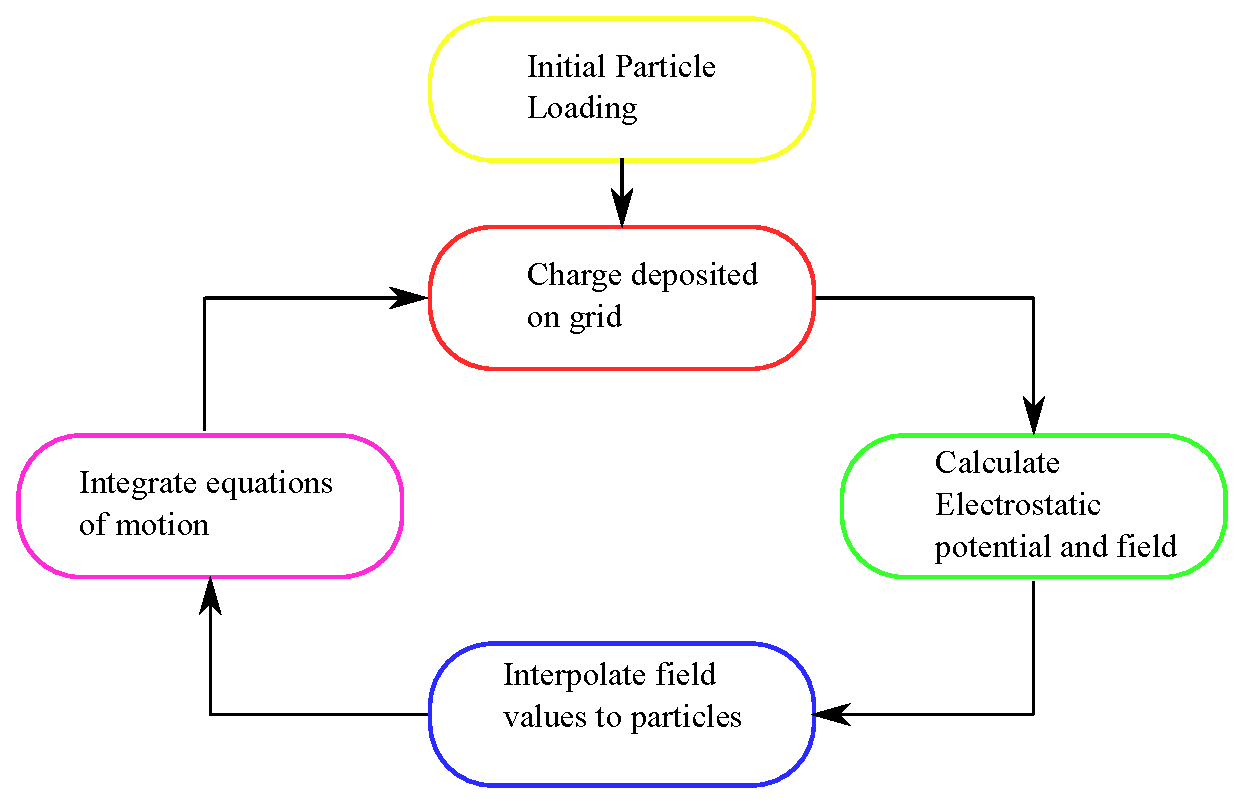
\includegraphics[width=0.8\textwidth]{piccycle}
\caption{A flow chart of the PIC algorithm \cite{loop}}
\label{fig:Leapfrog}
\end{figure}


%"A proper understanding of the sheath phenomena is also an important prerequisite for obtaining boundary conditions for fluid codes simulating tokamaks."
\subsubsection{Calculating the Density}
As discussed before particles are free to take any position along the domain and their positions determine the amount of charge they contribute to the grid points nearest them. Different weighting schemes can be used, some more accurate(less noisy) than others but at the expense of longer computation time. Weighting is the name given to how the charge density on the discrete grid points is distributed and also how the force exerted on the particles from the grid points is then calculated. The simplest weighting method is the Nearest Grid Point (NGP) scheme. This is a zero order weighting method in which the entirety of the particles charge is assigned to the grid point which it is closest to. Any particles within half a cell of the grid point are assigned to that grid point. Let the cell width be $\Delta x$, $x$ the distance from the grid point and $W(X)$ denote the weighting at grid point $X$. In the NGP scheme 

\be
    W(x)=
    \begin{cases}
      1, & \text{if}\ x \leq \frac{\Delta x }{2}   \\
      0, & \text{otherwise}
    \end{cases}
\ee

This is a computationally fast weighting method as it only requires one grid point look up per particle. As a particle moves away from a grid point and into the region of another grid point the grid density at that grid point jumps up to have a value of one and the grid point it just left falls down to 0. This gives the particle an effective shape, in this case rectangular. The particle also has a finite size of width $\Delta x$. Finite sized particles are a direct result of weighting particles on to the grid. The weighting method determines the effective size and shape of the particle as viewed by grid. Due to the large jumps to grid values caused by the movement of particles from one grid point to the next, the NGP weighting method is a large source of noise in the density and field calculations. A less noisy method is desired. 

\begin{figure}[H]
\centering
\includegraphics[width=0.8\textwidth]{particleshape}
\caption{The effective shape of a particle at position x as seen by the grid.\cite{shape}}
\label{fig:shape}
\end{figure}
First order weighting also known as the Cloud In Cell (CIC) method smooths the density and field fluctuations compared to NGP but is more computationally expensive as it requires two grid point look-ups for each particle. In this method each particle contributes charge to its nearest two grid points. The first step calculates the offset of the particle from the closest grid point to its left. 
\be
offset = x_i - X_j 
\ee 
where $x_i$ is the particles position and $X_j$ the grid point. $x_i > X_j$ always. The charge assigned to the $J^{th}$ grid point is then 
\be 
q_j = q_c \left(1 - offset\right)
\ee 
where $q_c$ is the charge of the particle. 
The charge assigned to the J+1 cell is 
\be 
q_{j+1} = q_c \left(offset\right)
\ee 
This results in a much smoother contribution to the density as the particle moves through the grid. The weighting puts the fraction of the clouds charge which is in the $J^{th}$ cell to the $X_J$ grid point and the rest of it goes to the $X_{J+1}$ grid point. This  gives the particle a triangular shape, so the particle is effectively a triangular cloud of uniform charge centred at $x_i$ with a width of $2\Delta x$ as it is able to influence a grid point from both sides of it. 

Higher order weighting methods do exist such as quadratic and cubic splines, that are second order and third order accurate respectively. These schemes further smooth the non-physical noise at the expense of more computation time by increasing the number of grid points that a particle contributes its charge to. This does lead to problems at the edge of the boundary where there are insufficient neighbouring grid points. It is unlikely that the NGP is in use in any of todays PIC codes due to the noise levels caused by interpolation but CIC is adequate for a lot of codes.

Use this for picutre %http://porl2.tripod.com/sitebuildercontent/sitebuilderfiles/mphysproject.pdf
\subsubsection{Calculating the Potential}
The potential can now be calculated from the known charge density at every grid point by solving Poisson's equation \eqref{eq:poisson}. This can be solved numerically by a computer using the Finite Difference Method (FDM). FDM solves differential equations via the discretisation of its derivatives. The first step is to carry out a Taylor series expansion of the potential, first in the forward direction.
\be
\psi(x+\Delta x) = \psi(x) + \Delta x \frac{\partial \psi}{\partial x} + \frac{{(\Delta x)}^2}{2}\frac{{\partial}^2\psi}{\partial x^2} + ...
\label{eq:forward}
\ee
The same procedure can be applied in the backwards direction 
\be
\psi(x-\Delta x) = \psi(x) - \Delta x \frac{\partial \psi}{\partial x} + \frac{{(\Delta x)}^2}{2}\frac{{\partial}^2\psi}{\partial x^2} + ...
\label{eq:backward}
\ee
These two equations can be used to give an approximate value for the second derivative of potential. Adding \eqref{eq:forward} and \eqref{eq:backward} with some rearranging gives 
\be 
\frac{{\partial}^2\psi}{\partial x^2} = \frac{\psi(x+\Delta x) -2\psi(x) + \psi(x-\Delta x)}{{(\Delta x)}^2}
\label{eq:phisolver}
\ee 
In FDM the solution to the equation is only known at the grid points, the potential is no longer a continuous function. Combining the forward difference and backward difference solution like this is known as central differencing and is second order accurate. For clarity we rewrite \eqref{eq:phisolver} with labels based on the grid number $j$. 
\be 
\frac{{\partial}^2\psi}{\partial x^2} = \frac{\psi_{j+1} -2\psi_{j} + \psi_{j-1}}{{(\Delta x)}^2} = -\frac{\rho_j}{\epsilon_0}
\label{eq:phisolver1}
\ee 

The value of $\psi$ at grid point j, ($\psi_j$),  depends on the value of $\psi$ at the two grid points either side of it $(\psi_{j-1}$ and $\psi_{j+1})$, so the grid points are coupled together. In order to find the value of $\psi_j$ at $N$ different grid points requires the solution of $N$ coupled linear equations. 


These coupled equations can be expressed in matrix form. 
\be
\begin{pmatrix}
  B_{1} & C_{1}  \\
  A_{2} & B_{2} & C_2 \\
        & A_3  & B_3 & C_3   \\
        & & \ddots & \ddots & \ddots \\
        & & &  A_N & B_N
\end{pmatrix}
\begin{pmatrix} 
 \psi_1  \\ 
 \psi_2  \\ 
 \psi_3  \\ 
 \vdots  \\
 \psi_N
\end{pmatrix}
= 
\begin{pmatrix} 
 \rho_1  \\ 
 \rho_2  \\ 
 \rho_3  \\ 
 \vdots  \\
 \rho_N
\end{pmatrix}
\ee
Where $A=1, B=-2$ and $C=1$. A matrix like this with non-zero elements only on the diagonal and one place either side of it is known as a tri-diagonal matrix.  The value of $\rho$ at each grid point is known as it was calculated in the previous step of the PIC algorithm. This matrix equation must now be solved in order to obtain the potential at each grid point. Plenty of tri-diagonal matrix solvers exist including the tridag solver found in Numerical Recipes\cite{NumericalRecipes}. Before this can be done the boundary conditions must be supplied. The first and last grid points only have one neighbouring grid point and so the previous equation no longer holds. Two common choices for boundary conditions exist, Dirichlet boundary conditions where $\psi_1$ and $\psi_N$ are set to a fixed value or Neumann boundary conditions where the gradient of the potential is fixed at the boundary. 
The implementation of Dirichlet boundary conditions is simple, $B_1$ and $B_N$ are set equal to one and $\psi_1$ and $\psi_N$ are then given the desired potential boundary values $\alpha $ and $\beta$  respectively. The first and last matrix equations then read
\be 
1.\psi_1 + 0.\psi_2 = \alpha 
\ee 
\be 
0.\psi_{N-1} + 1.\psi_N = \beta 
\ee 

Neumann boundary conditions involve fixing the gradient of the potential(i.e. the electric field) at the edge of the domain. This could be implemented by setting $B_1  = -\frac{1}{\Delta x}$, $C_1 = \frac{1}{\Delta x}$ and $\rho_1$ = $\alpha$. Thus giving the first line in the matrix equation as 
\be 
\frac{\psi_2 - \psi_1}{\Delta x} = \alpha 
\ee 

Once the boundary conditions have been supplied the tri-diagonal matrix equation can be solved.
 

\subsubsection{Calculating the Electric Field}
Once the potential is known at each grid point the electric field is easily found by calculating the gradient of the potential.
\be 
E = - \nabla \psi
\ee 
which in one dimension becomes
\be 
E = - \frac{\partial \psi}{\partial x}
\label{eq:electricfield}
\ee
This can discretised as before using the central difference method. 
\be 
E_J = - \frac{\psi_{J+1} - \psi_{J-1}}{2 \Delta x}
\ee 
Central differencing is not applicable at the boundaries due to a lack of neighbouring grid points and so either the forward or backward difference method must be used which is only accurate to first order. This provides the following two conditions to calculate the electric field at the edge of the domain.
\be
E_0 = - \frac{\psi_{J+1}-\psi_0}{\Delta x}
\ee 
\be 
E_N = - \frac{\psi_N - \psi_{N-1}}{\Delta x}
\ee
Using a first order equation at the boundaries reduces the accuracy throughout the solution to first order. Fortunately the accuracy can be improved to second order by carrying out a further Taylor expansion 
\be
\psi(x+2\Delta x) = \psi(x) + 2\Delta x \frac{\partial \psi}{\partial x} + \frac{{(2\Delta x)}^2}{2}\frac{{\partial}^2\psi}{\partial x^2} + ...
\label{eq:forward2}
\ee
Combining equations \eqref{eq:forward} , \eqref{eq:forward2} and \eqref{eq:electricfield} gives 
\be 
E_0 = \frac{3\psi_0 + \psi_2 - 4\psi_1}{2\Delta x}
\ee 
The exact same method in the backwards direction gives 
\be 
E_N = \frac{4\psi_{N-1} - \psi_{N-2} - 3\psi_N}{2\Delta x}
\ee
The second order boundary conditions restore second order accuracy across the domain.
\subsubsection{The Particle Mover}
The final step in the PIC cycle is to move the particles which requires calculating a new position and velocity for each particle in the simulation based on the forces acting on them. In order to do this Newtons equations of motion must be solved 
\be 
\vec{F}  = m \frac{d \vec{v}}{d t}
\ee 
\be 
\vec{v} = \frac{d \vec{x}}{d t}
\label{eq:diff2}
\ee 

Ignoring the presence of a magnetic field for now and limiting to one dimension gives the following equation of motion.
\be 
\frac{d \vec{v(x)}}{d t} = \frac{q}{m} E(x)
\label{eq:diff1}
\ee

The particles positions and velocities can be found by integrating the differential equations \eqref{eq:diff2} and \eqref{eq:diff1}. There are many ways in which these equations can be integrated, the methods vary in their complexity to implement as well as run time and accuracy. Depending on the needs of the simulator, a trade off may need to be made between fast run time and high accuracy. 

The simplest method of integration is Euler's method.
The finite difference method is used again to discretise the equations. 
\be 
v_{t+\Delta t} = v_t + \frac{dv}{dt} \Delta t + \frac{d^2v}{dt^2} {(\Delta t)}^2 + ...
\ee
\be 
x_{t+\Delta t} = x_t + \frac{dx}{dt} \Delta t + \frac{d^2x}{dt^2} {(\Delta t)}^2 + ...
\ee

In the Euler method The largest term neglected is $\propto {(\Delta t)}^2$. After taking $N$ steps where $N = \frac{total time}{\Delta t}$ the error is now proportional to $\Delta t$. For the case of charged particles moving in an electric field the equations of motion can now be written as
\be
v_{t+1} = v_t + \frac{qE}{m} \Delta t
\label{eq:accelerate}
\ee
\be 
x_{t+1} = x_t + v_t \Delta t
\label{eq:move}
\ee 
The field has been solved already in the previous step of the PIC cycle so $E$ is known. This is then used to accelerate the particle to a new velocity \eqref{eq:accelerate}. The new velocity is then used to find a new position \eqref{eq:move}. All particles are given an initial position and velocity at the start of the simulation so $x_0$ and $v_0$ are known.  The Euler method is very simple to implement and fast to run but is only first order accurate.

To demonstrate the stability of the Euler method it will now be applied to the case of a mass on a spring with equation of motion 
\be 
\frac{d^2 x}{dt^2} = -\frac{k}{m} x 
\ee
where $k$ is the Stiffness constant of the spring and $m$ is the mass of the attached object. An initial value for the position and velocity is required e.g. $v=1, x=0$.  Euler's method would approximate the equations of motion as 
\be
v_{t+1} = v_t - \frac{k}{m} x \Delta t 
\ee
\be 
x_{t+1} = x_t + v_t \Delta t
\ee
These equations can be solved multiple times to advance the system from its initial state. To check the accuracy of the Euler method the results are compared to the known analytical solution. 
\begin{figure}[H]
\centering
\includegraphics[width=0.8\textwidth]{Euler}
\caption{Euler solution to harmonic oscillator compared to analytical solution.}
\label{fig:E}
\end{figure}
The Euler method is unstable and quickly diverges from the analytical solution. This is no surprise based on the simplicity of the method. A more stable, higher order accurate integrator is desired for use in PIC codes.  Euler's method is described as an Explicit method as it uses the state of the system at the current time step to advance the system to its next time state. Implicit methods on the other hand use both the state of the system at the current time and the state of the system at the next time step to evolve the state of the system. An example of this is the Backwards Euler method. In this case the value of the velocity at time $t$ can be expressed as 
\be
v_t = v_{t+1 -\Delta t} = v_{t+1} - \Delta t \frac{dy}{dt}\Bigr|_{\substack{t=t+1}}
\ee
using a backwards Taylor expansion. Rearranging gives 
\be 
v_{t+1} = v_t +  \Delta t \frac{dy}{dt}\Bigr|_{\substack{t=t+1}} 
\ee 
A similar expression is found by replacing $v$ with $x$. Applying this to the case of the simple harmonic oscillator 
\be 
v_{t+1} = v_t - \Delta t\frac{k}{m} x_{t+1} 
\ee 
\be 
x_{t+1} = x_t - \Delta t\frac{k}{m} v_{t+1} 
\ee
The new value of the variable no longer depends on two known values as in the case of the Euler method but now depends on an unknown value from the next time step. It can be solved using the Newton-Raphson method. Implicit schemes are stable but more computationally expensive, this can be offset by the fact they allow for larger time steps to be taken and so can evolve a system to a desired time using less time steps than an explicit scheme. The stability of the numerical methods is not the only thing that limits the size of the time step in PIC codes, the size of the timestep is limited by the natural frequencies of the system \cite{Hockney1981}. This will be discussed more in the practical considerations section. The computational expensive and the need to use small time steps often rules out the use of implicit methods for the particle mover of PIC codes. 


Fortunately a more stable, explicit  method exists that is very similar to the Euler method and requires the same number of computations per time step but also has the advantage of being second order accurate. The Leapfrog method expands upon the Euler method. Instead of using the velocity at the beginning of the time step to advance the position it uses an average value of velocity throughout the time step. The leap-frog method involves offsetting the velocity by half a time step from the position. So the velocity of the particles is only known at half integer time steps while the positions are known at integer time steps. 
\be 
v_{t+1/2} = v_{t- 1/2} + \frac{qE_t}{m} \Delta t
\ee
\be 
x_{t+1} = x_{t} + v_{t+1/2} \Delta t
\ee 
This requires the initial velocities of the particles to be moved back half a time step at the beginning of the simulation, a "de-acceleration", in order to have time centred velocities. This just requires calculating the fields as before. This method is known as Leap-frog because in order to calculate new positions requires a leap over the known velocity. 

\begin{figure}[H]
\centering
\includegraphics[width=0.8\textwidth]{Leapfrog}
\caption{A graphical representation of the Leap-Frog scheme\cite{shape}}
\label{fig:Leapfrog}
\end{figure}
Instead of using the velocity at time $t$ to move the particle from $t$ to $t+1$ like the Euler method, Leap frog uses the velocity at time $t+\frac{1}{2}$ i.e. the average velocity of the particle between those two times. This method is more accurate than Euler's method for the same computational expense. The only extra step involves pushing back the particles half a time step but this only needs to be carried out once. For this reason Leap-frog is always the preferred choice over Euler and it can be proven to be second order accurate \cite{second_order}.
This method can also be applied to the case of the mass on a spring as before and compared to the analytical solution.
\begin{figure}[H]
\centering
\includegraphics[width=0.8\textwidth]{leapfrog}
\caption{A comparison of the numerical solution to the problem of a mass on a spring using the leapfrog method compared to the analytical solution.}
\end{figure}
This was run with as many time steps as Euler. It is clearly more stable. As with all explicit methods there exists a critical time step size, exceeding this leads to numerical instabilities. In the case of leapfrog $w dt <2 $ where $w$ is the highest frequency in the problem, usually the electron plasma frequency. COULD PROVE THIS WITH THE HARMONIC OSCILLATOR. However as mentioned before there are other factors which force the time step to be small for PIC codes so this is not a disadvantage to the Leap Frog method.
%Another method commonly used is the Runge Kutta method which involves Taylor expanding around both the current time point and the next time point WRITE THIS
%good link for code testing http://www.google.co.uk/url?sa=t&rct=j&q=&esrc=s&source=web&cd=1&ved=0CDEQFjAA&url=http%3A%2F%2Firfu.cea.fr%2FPhocea%2Ffile.php%3Fclass%3Dstd%26%26file%3DDoc%2FPublications%2FArchives%2Fdapnia-06-205.pdf&ei=y_OFU4OwN_Cd0wXRoIC4Bw&usg=AFQjCNFd2QEIIUKQkumEjvziFLLgv-wnGQ&sig2=v2eyb4zdTJSZ64rBXaQupA&bvm=bv.67720277,d.d2k"The second conventional test is a free drift of charged particles through the matter. The
%major task of the test is a verification of energy conservation with time because the use of the
%same weighting functions for charge and force approximations ensures only momentum
%conservation."  
%The problem with the Forward Difference method arises from the fact that it uses velocity at time “n” to push the particle from “n” to “n+1″. What makes more physical sense is to use the average velocity, the velocity that would exist at time “n+1/2″. This is the premise of the leapfrog method. Velocity and position integration leap over each other, being displaced by half a time step. This is illustrated in Figure 2 below (this same figure was used in the article on the particle in cell method). In our implementation, particle positions exist at the integral time steps, while velocity exists at the half times. This introduces little difficulty into particle loading, since source sampling will result in velocity and position at the same time step. The usual method is integrate the velocity (but not position) of all newly loaded particles backwards through -0.5dt. The implementation then follows:
%http://www.particleincell.com/blog/2011/velocity-integration/ 
%FORWARD DIFFERNCE DOESNT CONSERVE ENERGY , could try in my code? 
%
%good website for weak and strong coupling%https://perswww.kuleuven.be/~u0052182/pic/book.pdf
%
%
%"For strongly coupled systems, where the number of par-
%ticles per Debye cube is small, the PP approach is feasible" 
%
%REALLY GOOD http://www.daniel-martin.co.uk/files/pic.pdf
\subsubsection{Diagnostics}
Talk about the diagnostics capable of outputting, Talk about K.E using old and new velocities , what is the advantage of doing that. At waht time is the KE now known?
\subsubsection{Practical considerations}
ALiasing - Bottom of this %http://www.sciencedirect.com/science/article/pii/0021999170900495 


Noise One of these problems is that of “enhanced noise,” which arises because one is trying to simulate a system of %10 ^ 20 particles with 10^4. The
fluctuations generated by correlations are thus greatly magnified over the situation
in a real plasma. This aspect of the situation has been treated elsewhere [2] and
no further discussion will be directed towards it. C.K Birdsall and D fuss 1969 J. Computational Phys 





SOURCE OF ERRORS> ROUNDOFF ERRORS CHAPTER 4 in PARTICLE BOOK 
Timing errors can arise in PIC codes due to the discretisation of time which can cause a particle to leave its grid cell late and so arrive at the next grid cell also at the wrong time \cite{Birdsall1997141}. As time advances in fixed steps of $\Delta t$ a particle can only make the transition between cells at the end of a time step. If the particles average velocity in the cell is such that it would arrive at the end of the cell before the next increment of $\Delta t$ then the particle has effectively stayed in the cell for too long, the charge density at this grid point will be higher than expected and the density at the adjacent grid point will be lower than it should be. This effect is reduced by having many particles in a cell so that on average just as many particles leave a cell late as enter it late which acts to balance the incorrect charge density. The effect is also reduced by using higher order weighting schemes as the charge density is then assigned to multiple grid points. 

As alluded to in the previous section there are other considerations in PIC codes that limit the size of the time step. In order for the system to remain stable the Courant criterion must be met. This states that 
\be 
\Delta t < \frac{\Delta x }{v}
\ee
where $v$ is the fastest speed of propagation of a particle in the system. This prevents a particle from travelling across more than one grid point per time step. This is an important requirement as particles move due to the fields exerted on them. These fields are only calculated at the grid points and in the case of first order weighting a particle will only experience a force from the two grid points it is in between. If particles were able to move across multiple grid points in a single time step the particle would move based on the forces it experienced while in its original grid point and would not be affected by the fields in the other grid points it moves through. This could have important effects for example in the region of the sheath where there are strong electric fields. a particle allowed to move across multiple cells could potentially bypass the entire sheath without feeling a force if the time step were large enough. 


The particles used in PIC simulations are referred to as super particles as they represent hundreds of thousands, possibly more , of real particles. Although the mass and charge of the super particle is higher than that of the real particle it represents, the charge to mass ratio is the same and therefore a super particle will follow the same trajectory as that of a real particle. 

The use of a grid gives particles a finite size with a shape which depends on the weighting scheme used. So the super particles are in fact a cloud of charge moving through the domain. These super particles behave differently to point particles. As two super particles approach each other the force they exert on each other goes to zero rather than infinity like it would do for point particles. The grid effectively reduces the short range forces between particles which would otherwise be artificially enhanced by the small number of simulation particles used in simulations, so it is able to capture the same physics as reality by using less particles.



talk more about finite sized particles, 
time restrictions,
grid restrictions, 
noise , 
strongly coupled/ weakly coupled. 
different weighting, self force etc

"The use of
temporal and spatial grids, which are mathematical and not phy
sical, causes
concern about accuracy and may create "unphysical effects".
\subsection{Specific Boundary Conditions}
In order to model the case of a Langmuir probe I use a floating boundary condition on the right hand side of the domain, however to test the code to ensure every stage is in order it is much easier to use a double periodic system in which both ends of the domain have periodic boundary conditions. This section will detail the changes to the code required to make it periodic or floating. 

\subsubsection{Periodic Case}
In the periodic case the first grid point on the domain is $x_0$ and the last one is $x_{N-1}$ where N is the number of grid points. A particle travelling from left to right that goes past grid point $x_{N-1}$ will be on its way to travelling back to grid point $x_0$. So the length of the system is actually $L=N*dx$. Maybe get a dashed diagram. A periodic system represents an infinite length of plasma and so changes need to be made to the kill particle function in order to place a particle whose position exceeds $L$ back to the start of the domain and vice versa. Changes also need to be made to the calculate density function for a particle that lies in the last grid cell. The grid point on its left is the last grid point of the domain but the grid point on its right is the first grid point of the system so the right amount of charge needs to be deposited on the first grid point.  

A periodic system is defined such that $G_0 = G_{0+L}$ where $G$ is any grid value such as charge density or magnitude of electric field. This means $\psi_0 = \psi_L = \psi_N$ , $\psi_1 = \psi_{L+1}$ etc. At the boundaries \eqref{phisolver1} becomes 
\be 
\frac{\psi_1 - 2\psi_0 + \psi_{N-1}}{(\Delta x)^2} = - \frac{\rho_0}{\epsilon_0}
\ee
on the left hand side and 
\be 
\frac{\psi_0 - 2\psi_{N-1} + \psi_{N-2}}{(\Delta x)^2} = - \frac{\rho_{N-1}}{\epsilon_0}
\ee
on the right. This changes the matrix that must be solved. 
\be
\begin{pmatrix}
  -2 & 1 & & & 1  \\
  1 & -2 & 1 \\
        & 1 & -2 & 1   \\
        & & \ddots & \ddots & \ddots \\
        1 & & & 1 & -2
\end{pmatrix}
\begin{pmatrix} 
 \psi_0  \\ 
 \psi_1  \\ 
 \psi_2  \\ 
 \vdots  \\
 \psi_{N-1}
\end{pmatrix}
= 
\begin{pmatrix} 
 \rho_0  \\ 
 \rho_1 \\ 
 \rho_2  \\ 
 \vdots  \\
 \rho_{N-1}
\end{pmatrix}
\ee
In the case of a doubly periodic model it is not possible to use a direct matrix solver to solve this matrix. Any solution ($U$) that exists for the equation  can be combined with a constant ($U+C$) which will also be a solution to the matrix equation with those boundary conditions. The result of not having a unique solutions means the matrix is singular and doesn't have a unique inverse, as a result a direct matrix solver will fail. Fortunately an alternative method exists for periodic systems which is to use a discrete Fourier series for all grid quantities. This method relies on the assumption that $\rho(x)$ and $\psi(x)$ have Fourier transforms $\rho(\underline{\bold{k}})$ and $\psi(\underline{\bold{k}})$ where $\underline{\bold{k}}$ is the wavevector. The benefit of this method is that it provides spectral information on the grid quantities which enables easy comparison with plasma theory. The discrete Fourier transform of a grid quantity is given by 
\be 
G(k) = \Delta x \sum\limits_{j=0}^{N-1} G(X_j)e^{-ikX_j}
\ee 
and the inverse transform is given by 
\be 
G(X_j) = \frac{1}{L} \sum\limits_{n=-N/2}^{N/2-1} G(k) e^{ikX_j}
\ee 
The first step is to Fourier transform $\rho(x) \rightarrow \rho(k)$ using a Fast Fourier Transform (FFT). In 1d the differential of Poissons equation is replaced by $-k^2$ 
\be 
\psi(k) = \frac{\rho(k)}{\epsilon_0 k^2}
\ee 
This can now be used to solve for $\psi_k$. An inverse FFT will then convert  $\psi(k) \rightarrow \psi(x)$. The potential at each grid point is now known.
\subsection{Self Force}
The presence of the spatial grid introduces some non-physics into the simulation, an example of which is the self force. The self force is the name given to the phenomenon in which a charged particle becomes aware of its own field and so repels itself. This non-physical force is inherent in any system that uses the spatial grid to work out charge density and electric field values. Imagine a charged particle placed in between two grid points, let the particle reside closer to the left grid point to begin with. Using the first order weighting scheme (CIC) the particle will deposit more of its charge on to the left grid point than it will on to the right. This density will then be used to work out a potential and finally a field which is then interpolated back to the particles position, not necessarily using the same weighting scheme but for now consider it is the same. The particle will feel a larger force from the grid point on its left than it will do from the grid point on its right due to the relative distances and as a result it will be repelled from the left grid point and head towards the right. Although this argument assumed a first order weighting scheme, the self force is present with any method of weighting. 
It is possible to prove that the self force is introduced by the addition of a spatial grid rather than from any approximations made in using finite difference methods to solve Poissons equation. The following method is adapted from the textbook 'Numerical particle-in-cell Methods: Theory and Applications' \cite{selfforce}. 

The electric potential due to a point charge with charge $q$ at a distance $r$ is given by 
\be 
\psi = \frac{1}{4 \pi \epsilon_0} \frac{q}{r} = \frac{C q}{r}
\label{exact_potential}
\ee 
where $C$ is a constant. Now introduce a spatial grid with spacing $dx$. Let the particle be a distance $r$ from the grid point on the left and so a distance $dx - r$ from the point on the right. The particle will deposit a charge $\rho_1$ on the left grid point and a charge $\rho_2$ on the right where
\be 
\rho_1 = q\frac{(dx-r)}{dx}
\ee 
and
\be 
\rho_2 = q\frac{r}{dx}
\ee 
The particle will feel a potential that is a combination of the potential from the two grid points. From \eqref{exact_potential}the potential at the particle is 
\be 
\frac{C q}{dx} \left(\frac{dx - r}{r} + \frac{r}{dx - r} \right) 
\ee 
The force at the particle is given by 
\be 
F = -\frac{\partial \psi}{\partial r} q = Cq^2 dx\frac{dx-2r}{r^2(dx-r)^2}
\ee 
Despite the potential and electric field having been solved exactly without finite difference methods there still exists a self force due to the introduction of a spatial grid. This force is zero if the particle is at the midpoint of a cell ($r=\frac{dx}{2}$) and acts to repel the particle from its closest grid point.

It is possible to quantify this force in the case of a complete PIC simulation where FDM are used. As before Poisson's equation is discretised 
\be 
-\rho_J = \frac{\psi_{J+1} - 2\psi_J + \psi_{J-1}}{(dx)^2}
\ee 
This equation can be solved analytically without a matrix equation.
\be 
\psi_J = \frac{I-J}{I} A + \frac{J}{I} B + \frac{dx^2}{I} \left[(I-J) \sum\limits_{k=1}^J k\rho_k   + J \sum\limits_{k=J+1}^{I-1} (I-k)\rho_k \right]
\label{potential_analyitical}
\ee
Where $I$ is the number of the grid cells , $A$ is the potential at the left hand side boundary and $B$ the potential at the right hand side. 
This will now be carried out for one particle. Let the particle lie between grid points $x_{\alpha -1}$ and $x_\alpha$ at position $x$. The offset ($\sigma$) is given by 
\be 
\sigma = \frac{x - x_{\alpha -1}}{dx}
\ee
Using \eqref{potential_analyitical} it is possible to calculate the potential at the grid points either side of the particle. 
\be
\psi_\alpha  = \frac{I-\alpha}{I}A +\frac{\alpha}{I}B - \frac{dx^2}{I}(I-\alpha) \left[(\alpha-1)\rho_{\alpha-1} + \alpha \rho_{\alpha} \right]
\ee
\be 
\psi_{\alpha -1} = \frac{I-\alpha +1}{I}A + \frac{\alpha - 1}{I} B -\frac{dx^2}{I}(\alpha -1) \left[(I-\alpha +1)\rho_{\alpha -1} + (I-\alpha)\rho_\alpha \right] 
\ee
Similar expressions can be derived for $\psi_{\alpha+1}$ and $\psi_{\alpha-2}$. These can then be used to derive the value of the electric field at the adjacent grid points. 
\be 
E_\alpha = \frac{\psi_{\alpha -1} - \psi_{\alpha +1}}{2 dx} = \frac{A-B}{I dx} - \frac{dx}{I}\left[(\alpha -1) \rho_{\alpha -1} + (\alpha -\frac{I}{2})\rho_\alpha \right]
\ee 
\be 
E_{\alpha-1} = \frac{\psi_{\alpha -2} - \psi_\alpha}{2 dx} = \frac{A-B}{I dx} - \frac{dx}{I} \left[(\alpha-\frac{I}{2}-1) \rho_{\alpha -1} +(\alpha-I) \rho_\alpha \right] 
\ee
Using the first order weighting method, the force at the particle $E_i$ will be given by 
\be 
E_i = E_{\alpha -1 } (1-\sigma) + \sigma E_\alpha = \frac{A - B}{I dx} - \frac{dx}{I} \left[(\alpha -\frac{I}{2} -1 + \frac{I}{2} \sigma) \rho_{\alpha -1} + (\alpha -I +\frac{I}{2} \sigma) \rho_\alpha \right]
\ee
The self force is inherent in PIC codes and always acts to repel a particle from its nearest grid point going to zero when the particle is at the midpoint of a grid cell. Interestingly this equation shows the impact that boundary conditions have on the self force. The force not only depends on the location of the particle in the grid cell but also in which cell it lies in. Provided there are sufficient amount of particles the self force will be negligible. 


\subsubsection{Talk about the Code I have developed}
Talk about your code, what it does, what it assumes, what physics is in it, what could be added. 
Maxwellian test -particles injected with a maxwellian distribution, how, how was it tested, graph
Two stream test
Floating test 
Harmonic Oscillation test
\subsubsection{Tests}
\subsubsection{Cold Plasma Oscillations} 
It is well known that if electrons in a plasma are displaced from their equilibrium position they will feel a restoring force due to electric fields which will act to quickly return the electrons to their equilibrium position. Once they reach this equilibrium position their kinetic energy will cause the electrons to overshoot and so a cycle begins with electrons oscillating around their respective equilibrium positions. The time frequency at which these oscillations occur is called the plasma frequency ($\omega_p$). 
In a real plasma these oscillations are non-dispersive, the frequency the electrons will oscillate at is always the plasma frequency and does not depend on the initial amplitude or wave number of the displacement. This is not the case in a PIC simulation of the plasma, alias effects from the grid introduce a dispersion relation EXPAND ON THIS. The frequency the electrons will oscillate at now has a wave number dependence. 
\be 
\omega(k) = \omega_p cos\left(\frac{k \Delta x }{2} \right) 
\ee
$\omega(k)$ is the frequency that will be measured in PIC experiments. It is possible to measure this by plotting the kinetic energy of the electrons against time. As a first test a plot was made of kinetic energy and potential energy against time.
\begin{figure}[H]
\centering
\includegraphics[width=0.8\textwidth]{keandpe.png}
\caption{A plot of Kinetic energy and Potential Energy versus time. Shows the interchange of kinetic energy with potential energy}
\end{figure}
The electrons begin stationary with no kinetic energy. Their displacement gives them a potential energy which is converted into kinetic energy. The velocity has a sinusoidal dependence of time, the kinetic energy $(\tau)$ therefore obeys 
\be 
\tau = Asin^2(\omega_p t)
\ee
where $A$ is the amplitude. By fitting this curve to the plot of kinetic energy it is possible to determine 
$\omega_p$. This can be carried out for multiple wave numbers to see if the plasma frequency does have a  mode dependence. 

The code was set up with the following parameters. 
\begin{table}[h]
\begin{tabular}{lllll}
L  & ${2\pi}$      \\
GP & 512    \\
N  & 1024   \\
W  & 1e6   
\end{tabular}
\end{table} 
The code was ran with different modes ranging from 1 to 70. The plasma frequency was measured for each and the results are shown below along with the theoretical dispersion relation.
\begin{figure}[H]
\centering
\includegraphics[width=0.8\textwidth]{cold_results.png}
\caption{Dispersion Relation for the cold plasma oscillations both measured and theoretical}
\end{figure}
The two are in good agreement with each other thus demonstrating the aliasing effects of the grid. EXPAND ON THIS 


\subsubsection{Cold Beam Instability} 
The cold beam instability is a phenomenon found to occur in PIC codes but in reality the system is stable. During this instability an initially cold beam of electrons will heat up until a saturation temperature is reached, at which point the instability is quenched.  The electrons are initially given a uniform drift velocity $v_0$ and are uniformly distributed throughout the grid. The instability leads to an increase in thermal energy of the particles but not at an expense of their initial kinetic energy, as a result the total energy of the system increases due to this instability which is obviously an non-physical result. The instability is caused by an aliasing effect with the grid (EXPAND). Theory predicts the instability will stop once 
\be 
\frac{\Lambda_D }{\Delta x} = \frac{v_t}{w_p \Delta x} = 0.046
\label{eq:cold_beam}
\ee 
The effects of the instability are shown below. 
\begin{figure}    
\begin{minipage}[t]{0.45\textwidth}
\includegraphics[width=\linewidth]{KineticEnergy.png}
\caption{Actual Versus Predicted: Immediate}
\label{fig:immediate}
\end{minipage}
\hspace{\fill}
\begin{minipage}[t]{0.45\textwidth}
\includegraphics[width=\linewidth]{FieldEnergy.png}
\caption{Actual Versus Predicted: Proximal}
\label{fig:proximal}
\end{minipage}

\vspace*{0.5cm} % (or whatever vertical separation you prefer)
\begin{minipage}[t]{0.45\textwidth}
\includegraphics[width=\linewidth]{ThermalEnergy.png}
\caption{Actual Versus Predicted: Distal}
\label{fig:distal}
\end{minipage}
\hspace{\fill}
\begin{minipage}[t]{0.45\textwidth}
\includegraphics[width=\linewidth]{TotalEnergy.png}
\caption{Actual Versus Predicted: Combined}
\label{fig:combined}
\end{minipage}

\end{figure}
\newpage
The thermal energy of the beam rises until a critical temperature has been reached, at that point the instability abruptly stops and energy fluctuates but does not grow. To test the point of saturation simulations were run with my code keeping the length of the system the same but varying the number of grid points which is equivalent to changing $\Delta x$. In all runs the length of the system was $2\pi$ and the same number of particles were used with the same initial velocity. The thermal energy at saturation was used to determine the thermal velocity and this was then compared to \eqref{eq:cold_beam}. A coefficient of 0.049 was found to be the average result which is consistent with Berkley's XES1 code. The relation is an approximate one. Tests were also carried out on how the initial velocity of the electrons effected the thermal velocity at saturation, it was found not to have an effect which is consistent with theory.

As the instability stops once the temperature has reached thousands of an eV it is not likely that this instability will cause any problems in simulations that I will be doing, never the less this instability provided a useful test case on which to benchmark my code. Giving a temperature to the beam at the beginning of the simulation prevents the instability from occurring provided the beam temperature is higher than the saturation temperature.

%Paragraph on the difference between a 1D and 3d code, much more computation time etc. Do the field solving formula change and if so how.
\subsubsection{Review of Existing Pic Codes}
%Explain there are pic codes already out there that model the plasma edge. Can add probes to these codes and model their behaviour. 
Table of codes both commercial and open source. What would be useful for me, what isn;t useful. 

\section{Plasma Surface Interactions}
Understanding the interactions between plasmas and material surfaces is crucial in many areas of plasma science....% It is particularly relevant to probes because ... copy abstract of project or poster secondary e emission etc

The plasma sheath plays a vital role in probe theory so this will discussed first. 
\subsection{Sheath}

A plasma sheath forms whenever a material object comes into contact with a plasma e.g. a Langmuir probe inserted into the plasma or the containing wall of a tokamak. In the case where the wall is initially neutral, electrons in the plasma will rush to the wall ahead of the ions and hence give it a negative charge. This occurs because electrons are much less massive than ions and typically at a higher temperature and so move around much faster in the plasma. This process can not go on indefinitely. Due to the increasing negative charge on the wall a potential barrier builds up that begins to repels electrons and attracts ions \cite{sheathformation}. The potential barrier continues to increase reducing the electron flux and increasing the ion flux until a steady state is obtained once the two fluxes become equal. The potential of the wall at steady state is the floating potential $V_F$. The wall is said to be floating. 
\begin{figure}[H]
\centering
\includegraphics[width=0.8\textwidth]{stangebysheath}
\caption{A schematic of the variation of electric potential with distance from the wall in a plasma \cite{stangeby-2000}.}
\label{fig:stangebysheath}
\end{figure}
The sheath is a transition layer in the plasma between the floating material surface and the bulk plasma. In the sheath quasi-neutrality no longer holds, the plasma gains a positive space charge as ions are attracted towards the negative potential and the electrons repelled. This positive layer separates the rest of the plasma from the wall of the containing vessel and acts to shield the rest of the plasma from the negative potential. The sheath has a thickness on the order of 10 Debye lengths which corresponds to $\approx $ 10$ \mu m$ in a typical scrape off layer off a tokamak. % EXPLAIN DEBYE LENGTH, GET FORMULA, 
 It is possible to calculate the ion velocity at any point in the sheath by applying the principle of conservation of energy as demonstrated in this simple model.

For simplicity we will work in one dimension. The bulk plasma lies at the origin x=0, here quasi-neutrality holds and the potential $V=0$. The floating material surface lies at x=b and has a negative potential with respect to the plasma. 
By applying conservation of energy we know that the velocity of the ions $v(x)$ at any position is given by 
\be 
v(x) = v_0 \sqrt{1 - \frac{2 e V(x)}{m_i v_0^2}}
\ee
where $v_0$ is the initial velocity of the ions before entering the sheath and $m_i$ is the mass of the ions. 

The moving ions form an electric current density  
\be 
J_i = e n(x) v(x) = e n_0 v_0 
\ee
This is conserved so doesn't vary with position in the sheath. As a result of this the density of ions must decrease as we move in to the sheath to balance out the increase of speed as the ions accelerate towards the negative charge. The density in the sheath is given by 
\be 
n(x) = \frac{n_0 v_0 }{v(x)} = \frac{n_0}{\sqrt{1 - \frac{2 e V(x)}{m_i v_0^2}}}
\ee 
Assuming a Maxwellian distribution of electrons the electron density in the sheath is then described by the Boltzmann equation 
\be
n_e(x) = n_0 \exp \left(\frac{e V(x)}{k T_e}\right)
\label{eq:sheathdense}
\ee
This is an often used approximation as most electrons in the sheath are reflected by the negative wall and so oscillate back and forth through the sheath.
The densities can now be plugged in to Poisson's equation to solve for the potential 
\be
\frac{d^2 V}{dx^2} = \frac{e}{\epsilon_0} (n_e - n_i) =  \frac{e}{\epsilon_0} n_0 \left[exp \left(\frac{e V(x)}{k T_e}\right) - \frac{1}{\sqrt{1 - \frac{2 e V(x)}{m_i v_0^2}}} \right]
\label{eq:poisson}
\ee 
This can be simplified by normalising to dimensionless values. $\hat{x}$ denotes a normalised length.
\be 
\hat{V} = \frac{e V }{k T_e}, \;\; \hat{x} = \frac{x}{\lambda_D}, \;\; \hat{v_0} = \frac{v_0}{v_B} = \frac{v_0}{\sqrt{\frac{k T_e}{m_i}}}
\ee
where $v_B$ is the Bohm velocity. Expressed in terms of these variables the Poisson equation becomes
\be 
\frac{d^2 \hat{V}}{d \hat{x}^2} = \frac{1}{\lambda_D ^2} \left[\exp(\hat{V}) - \frac{1}{\sqrt{1 - \frac{2\hat{V}}{\hat{v_0^2}}}}\right]
\label{eq:normalisedpoisson}
\ee 
The right hand side of this equation is directly proportional to $n_e - n_i$. In the bulk plasma where $V=0$ the RHS = 0 as would be expected in a quasi-neutral plasma. As we approach the negative probe the electron density drops as does the ion density but at a slower rate.

By Taylor expanding the RHS we find 
\be 
n_e - n_i \approx (1 + \hat{V} + \frac{1}{2} \hat{V}^2 + ...) - (1 + \frac{1}{\hat{v_0}^2} \hat{V} + \frac{3}{2 \hat{v_0}^4} \hat{V^2} + ...)
\ee
which simplifies to
\be 
\left(1 - \frac{1}{\hat{v_0}^2}\right) V + \frac{1}{2}\left(1 - \frac{3}{\hat{v_0}^4} \right) V^2 
\ee
In order for a positive sheath to form around the negative probe the ion density must exceed the electron density meaning the RHS must be negative. This is true if $\hat{v_0}\ge 1$ or in real units $v_0 \ge v_B$. This is known as the Bohm criterion. In order for the equilibrium between the fluxes to be established, the ions must be moving at sufficient velocity above their thermal velocity before entering the sheath. This suggests a region beyond the sheath, a presheath, responsible for accelerating the ions up to the Bohm velocity before entering the sheath. The presheath is a quasi-neutral region that extends much further out in the plasma than the sheath. 

In order for this acceleration to occur a potential difference must exist between the sheath boundary and the bulk plasma. Let the potential in the bulk plasma be $V_{p}$ and the potential at the sheath boundary be $V_0$. The gain in kinetic energy of the ions as they move through the sheath is fuelled by a loss of potential energy. For simplification assume the ions are initially stationary, we then have 
\be
\frac{1}{2} m_i c_s^2 = e (V_{p} - V_0) 
\ee
Which can be rearranged to 
\be 
V_{s} - V_0 = -\frac{k T_i}{2 e}
\ee 
This allows us to determine the reduced density of ions at the sheath edge relative to that in the bulk plasma using \eqref{eq:sheathdense}
\be 
n_s = n_0 exp \left( \frac{-e(V_0 - V_s)}{k T_i}\right) = n_0 exp\left(-\frac{1}{2}\right) \approx 0.61 n_0
\label{eq:presheathdrop}
\ee


%An analytical solution exists for a one dimensional planar sheath and can be derived from Poisson's equation. 
%\be 
%\frac{d^2 V}{dx^2} = \frac{e}{\epsilon_0} (n_e - n_i)
%\ee 
%
%The origin is defined to be at the sheath edge between the presheath and the Debye sheath. At this point the potential is also defined to be zero. Underscore s values e.g.  $x_s$ denote the value at the sheath edge. 
%
%For Maxwellian electrons their density in the sheath region is given by 
%\be 
%n_e = n_s e^{\frac{eV}{k T_e}} = n_s e^{-\eta}
%\ee
%where 
%\be
%\eta = - \frac{eV}{k T_e}
%\ee 
%
%The density of ions can be determined by applying the principles of conservation of energy \eqref{eq:conenergy}  and continuity of ion flux  \eqref{eq:conflux}
%\be
%\frac{1}{2} m_i v_i^2 = \frac{1}{2} m_i c_s^2 - eV
%\label{eq:conenergy}
%\ee
%i.e an ion has a kinetic energy in the sheath equivalent to the kinetic energy it had when entering the sheath plus the potential energy it has lost.
%
%\be 
%n_i v_i = n_s c_s 
%\label{eq:conflux}
%\ee 
%
%Combining these two equations results in an equation for the density of the ions in the sheath 
%\be
%n_i = n_s \left(1 - \frac{2 e V }{m_i c_s^2} \right)^{- \frac{1}{2}} = n_s (1 + 2\eta)^{-\frac{1}{2}}
%\ee
%The values for $n_e$ and $n_i$ can now be plugged into Poissons equation to give 
%\be
%\frac{d^2 V}{d x^2} = \frac{e}{\epsilon_0} n_s \left[e^{-\eta} - (1 + 2\eta)^{-\frac{1}{2}} \right] = - \frac{k T_e}{e} \frac{d^2 \eta}{d x^2}
%\ee
%The equations can be simplied by normalising length scales with respect to the Debye length at the sheath edge 
%\be 
%\hat{x} = \frac{x}{\lambda_{D,s}}
%\ee 
%where the Debye length is given by
%\be
%\lambda_D = \sqrt{\frac{\epsilon_0 k T_e}{n_s e^2}}
%\ee
%This leads to the following equation 
%\be
%\frac{d^2 \eta}{d \hat{x}^2} = (1+ 2 \eta)^{-\frac{1}{2}} - e^{-\eta})
%\ee
Equation \eqref{eq:normalisedpoisson} can be solved analytically by providing boundary conditions for the electric field and potential at the sheath edge. 
\begin{figure}[H]
\centering
\includegraphics[width=0.8\textwidth]{graphofpotentialanddensity}
\caption{Analytical solution of Poisson's equation for a planar sheath.}
\label{fig:numericalsolution}
\end{figure}
This shows a sheath region of positive space charge a few Debye lengths thick. Before entering the sheath the density of the electrons is equal to that of the ions and the plasma potential is constant as the charge from the wall is screened out. A potential drop occurs in the sheath region as screening of the wall potential becomes less effective, reaching a maximum at the wall.

The thickness of the sheath depends on the assumed boundary conditions therefore a plane sheath does not have a unique thickness. The sheath edge conditions are  arbitrary and these control the sheath thickness. There is a current dispute as to where the sheath edge should be chosen \cite{0963-0252-18-1-014004}. 
The overall role of the sheath is to protect the wall from the plasma heat. Although the ion flux to the wall is increased by a factor of two by the presence of the sheath, the electron flux is reduced by a factor of 20 giving an overall reduction in flux of around an order of magnitude \cite{picmaster}.
%http://www.en-trust.at/eibl/wp-content/uploads/sites/3/2013/08/Eibl05_MSc_thesis_physics.pdf

\subsection{Sputtering}
\subsection{Secondary E emission}
%Read this http://www.en-trust.at/eibl/wp-content/uploads/sites/3/2013/08/Eibl05_MSc_thesis_physics.pdf 
\subsection{Thermionic emission}
\subsection{Chemical Erosion}
\section{Probe Theory}
\subsection{Introduction}
%The
%ability of a probe to simultaneously record information about plasma density, electron
%temperature,
%plasma potential and fluctuations of these quantities in a spatially
%localized
%region is
%virtually
%unsurpassed by
%any other diagnostic.
%However,
%these measurements come at a price;
%one must
%confront potential problems in interpreting the data: Can the measured quantities be reliably r
%elated
%to plasma parameters in the absence of the probe? To
%what
%degree are the inferred quantities being
%influenced by the presence of the
%probe and complications associated plasma-surface in
%teraction
%physics? Probe diagnosticians
%are
%usually
%well
%acquainted
%with
%such concerns. For
%example,
%corrections in electron temperature due to a non-thermal electron population and/or temperature
%gradients along
%magnetic field lines are
%well
%known
%1-4
%. The influence of the probe-induced
%presheath zone and its extent along magnetic field lines relative to nearby objects
%hasbeen analyzed
%extensively 5-7
%and measured in high density plasmas in some detail
%8-10. There is the additional constraint of power density limitations; if the electrodes become sufficiently hot then thermionic electron emission can interfere with data interpretation."
Langmuir probes are the oldest type of plasma diagnostic device and are still one of the most frequently employed tools used to obtain information about conditions inside a plasma. In relation to tokamaks Langmuir probes are the most reported edge diagnostic in the literature \cite{matthews}.The main advantage of using probes is that they can make highly localised measurements, almost all other diagnostics give volume averaged measurements. The probes take their name from the Nobel prize winning scientist Irving Langmuir who coined the term plasma and whose paper published in 1926 with H.M. Mott-Smith provided a means to measure plasma parameters by obtaining a Current-Voltage curve (IV curve) using a probe \cite{mottsmith}. The probe in its simplest form is a metallic electrode, electrically biased with respect to a reference electrode which is then inserted into a plasma to draw an ion or electron current. In the simplest case the electrode has a well defined geometry either planar, spherical or cylindrical. This set-up is known as the single probe. More sophisticated  designs do exist such as double and triple probes and will be discussed later in this report. Electrical probes are used to diagnose a wide range of plasmas from space plasmas with low-density and weak magnetic fields to those at the edge of nuclear fusion devices with hostile conditions to material surfaces and strong magnetic fields. The use of probes requires direct contact to be made between the probe and the plasma and so their use is limited by the conditions in which they can survive. This restricts the use of probes to the edge of tokamak devices where the plasma is less dense and cooler. 
\paragraph{}
Langmuir probes are a powerful diagnostic capable of providing local measurements of the plasma potential $(V_{p})$, electron density $(n_e)$ and electron temperature $(T_e)$ with a good time resolution of approximately $10^{-8}$ seconds \cite{probetheoryandpractise}. They are fairly easy to design and build and acquiring data from them is straightforward. Despite their simplicity in construction and operation, probes do have a downside compared to other diagnostics. As probes are in contact with the plasma, they perturb it, changing the local density and potential in the surrounding plasma. This complicates the interpretation of probe data. The role of probe theory is to determine the unperturbed values of the plasma which would exist in the absence of the probe. However theoretical models used to interpret the data can be very complicated and in some cases non-existent. No general model exists that is capable of relating the measured current voltage curves with the actual plasma properties under all possible physical conditions. An overview of the general probe method will be given followed by complications that arise especially in the presence of magnetic fields. 

\subsection{General Probe Method}
\paragraph{}
The method for obtaining probe data is relatively simple. The metallic electrode is immersed in plasma and then biased to a potential $V_B$ by an external circuit. The collected current $I_p$ is then recorded at different probe voltages allowing an IV curve to be recorded. The plasma parameters are then deduced from this IV characteristic.  Charged particles are drawn to the probe by its electric field which extends a few Debye lengths into the plasma, in the region known as the sheath. The theory developed by Langmuir and Mott-Smith allows the plasma parameters to be deduced for unmagnetised plasmas with a Maxwellian distribution of ions and electrons. This will be discussed before moving on to more complicated situations. 
\subsubsection{Ideal Probe Theory}
When a probe is inserted into a plasma it is bombarded by neutral particles and the charged electrons and ions. Absent of any electric forces the impact rate per $m^2$ for each species is given by their random thermal flux which can be expressed as 
\be 
\Gamma = \frac{1}{4} n \langle{v}\rangle 
\label{eq:thermalmotion}
\ee
where $n$ is the number density of that particular species and $\langle{v}\rangle$ the average speed. For a Maxwellian distribution of particles this can be expressed as 
\be 
\Gamma =  \frac{1}{4} n \sqrt{\frac{8 k T}{\pi M}}
\ee
Electrons are less massive than ions and tend to be hotter so if no bias voltage is applied to the probe, the probe is allowed to float and will quickly charge up negative until it reaches the floating potential $(V_F)$. At floating potential the probe collects zero net current from the plasma. It is less than the plasma potential $V_{p}$ as a negative bias is required to retard the flow of electrons and accelerate ions in order to balance the two fluxes.
\paragraph{}
During probe operation the probe voltage is swept from negative to positive while the current collected by the probe is recorded in order to produce the IV curve. Data for the entire curve can be obtained in a few microseconds by using a fast sweeping voltage source \cite{chen-notes}. The current collected by the probe will be composed of ions or electrons or a combination of both depending on the applied potential of the probe. For $V_B = V_F$ no net current is drawn from the plasma as the electron flux reaching the probe is balanced by the ion flux. For $V_B > V_F$ the electron flux exceeds the ion flux and therefore a net current will flow into the plasma while for $V_B <V_F$ ion flux exceeds electron flux therefore a net current flows out of the plasma. Typical sign convention declares current leaving the plasma as negative while current entering the plasma as positive. A typical ideal IV curve is shown below. The curve is described as ideal because it is a theoretical prediction of an IV curve in an unperturbed plasma. Experimental IV curves deviate from the ideal case, this will be detailed later in the report.
%\begin{figure}[H]
%\centering
%\includegraphics[width=0.8\textwidth]{idealcurve}
%\caption{A theoretical IV curve that would be obtained by a Langmuir probe in an ideal plasma}
%\label{fig:idealcurve}
%\end{figure} 
\begin{figure}[H]
\centering
\includegraphics[width=0.8\textwidth]{monkiv}
\caption{A schematic of the IV curve obtained with a single Langmuir probe \cite{monk}.}
\label{circuit}
\end{figure}

%http://iopscience.iop.org/0741-3335/37/11/011/pdf/0741-3335_37_11_011.pdf

\paragraph{}
The floating potential is labelled on the figure, at this point zero net current is drawn by the probe. While $V_B < V_{p}$ the probe is biased negative with respect to the plasma potential therefore ion collection to the probe is unhindered and so ions are collected at a saturated rate. If the probe bias is sufficiently negative all electrons are repelled and the current collected by the probe is then the ion saturation current approximated by the Bohm current 
\be 
I^{+}_{sat} = n_s e v_B A 
\label{eq:isat}
\ee
where $n_s$ is the ion density at the sheath edge, $e$ is the fundamental charge and $A$ the area of the exposed probe tip. This current arises due to the acceleration of the ions in the presheath. Equation \eqref{eq:presheathdrop} shows a decrease in the ion density at the sheath edge from that in the bulk plasma, we can therefore rewrite the ion saturation current in terms of bulk plasma parameters
\be
I^{+}_{sat} \approx 0.61 n_0 e v_B A
\ee
There are other theories for ion collection that allow the ion current to be calculated, these will be discussed later in the report. 
The ion flux is independent of the applied potential so making the probe more negative will not result in an increase in probe current. Having said that under some conditions the sheath will expand as probe voltage becomes more negative this increases the collection area of the probe and so the ion current does not saturate. This will be discussed further when we look at probes in real conditions.

As the bias voltage increases (becomes more positive) the sheath potential drop is reduced allowing electrons at the high energy tail of the distribution to reach the probe. This region of the curve is known as the transition region. As $V_p \to V_{p}$ more and more electrons are able to reach the probe as less kinetic energy is needed to overcome the potential. For a Maxwellian distribution of electrons and neglecting effects such as secondary electron emission, the electron current able to reach the probe is given by 
\be  
I^{-} = \frac{1}{4} n_0 e A \sqrt{\frac{8 k T_e}{\pi m_e}}  \exp\left[\frac{e(V_p-V_{p}}{k T_e}\right]
\label{eq:ecurrent}
\ee
The term $\sqrt{\frac{8 k T_e}{\pi m_e}}$ will be denoted as $c_e$ from now on. This is just the random thermal flux of the electrons reduced by the Boltzmann factor. The total current reaching the probe in this region will be made up of ions and electrons. The total current as a function of bias voltage is then 
\be 
I(V_B) = - n_0 e A\left(0.61 v_B - \frac{1}{4}  c_e \exp\left[\frac{e(V_p-V_{p}}{k T_e}\right] \right)
\ee
As the probe bias continues to rise it will eventually be equal to the plasma potential. At this point there are no electric fields as there is no potential difference between the probe and the plasma and so the sheath disappears. The charged particles now reach the surface of the probe due to their thermal motion and so the probe collects the thermal flux of both electrons and ions. No electrons are repelled any more. Increasing the potential of the probe will act to repel the ions and a negative sheath of electrons now forms around the positive probe to shield out the positive charge. This sheath is very thin and the electric field outside of it is again zero. The electron saturation current is then just the random thermal flux of electrons that enter the sheath
\be  
I^{-}_{sat} = \frac{1}{4} n_0 e c_e A
\label{eq:esat}
\ee
The curve has a sharp knee at this point where the collected current is no longer exponentially increasing. This sharp knee is often rounded in experimental curves.
For a pure hydrogenic plasma with no magnetic fields the ratio of the electron saturation current to ion saturation current is very high, it is typically found that 
\be 
\frac{I^{-}_{sat}}{I^{+}_{sat}} \approx 60
\ee
For this reason the ion contribution to the total current is negligible and often ignored. The total current reaching the probe when $V_B > V_{p}$ is then given by \eqref{eq:esat}. %An increase in the saturation current is noticed with increased applied voltage due to the sheath around the probe expanding. This acts to increase the effective collecting area of the probe. The shape of the resulting curve depends on the shape of the exposed probe tip. GET REFERENCE


By equating \eqref{eq:ecurrent}  and \eqref{eq:isat} a value for the floating potential is found. 
\be 
V_f = V_{p} - \frac{k T_e}{2 e} ln\left(2 \pi\frac{m_i}{m_e}\right)
\label{eq:floating}
\ee
In a pure hydrogenic plasma $V_f$ is typically found to be $\approx -3.5 T_e $. 
The above equations have all assumed the simplest case of a collisionless sheath with no magnetic field present. All surface-plasma interactions have been ignored. Also these equations are only valid for the thin sheath regime where the probe diameter $d$ $>>$ $\lambda_D$. In some cases (list) it is possible for a thick sheath regime to exist. In this case $\lambda_D >> d$. Due to their orbital motions around the probe, not all charged particles that enter the sheath will actually be collected by the probe. The current drawn by the probe is now a function of bias voltage and also depends on the detailed geometry of the probe. 

\subsubsection{How Measurements are made} 
After an IV curve has been obtained it must be interpreted in order to extract physical parameters of the plasma. Interpretation is difficult and requires the correct physical model to be applied that relates the collected current to the energy distribution function of charged particles. Each model makes certain assumptions about conditions in the plasma, these assumptions may be valid only in certain scenarios. The correct model depends on the plasma. The simplest case is a plasma with no magnetic field applied, no collisions between the particles and a Maxwellian distribution of velocities. This case is discussed below.  
\paragraph{}
By looking at equation \eqref{eq:esat} it would appear the that electron saturation current could be used to determine the electron density. However this region is rarely used in practise as the electron saturation current is so high. Probes that are left to collect the electron saturation current for more than a few milliseconds at a time will suffer damage from the large particle flux. Due to the lower fluxes involved, the ion saturation region is a more useful area for probe diagnostics. 
In the transition region where $V_F < V_B < V_{p} $ the IV curve obeys an exponential relationship as long as the electrons are Maxwellian. By plotting this region on a semi-log plot a straight line is obtained with gradient $\frac{1}{k_B T_e}$. The electron temperature is a fairly robust measurement and is the easiest one to obtain from the probe. Before carrying out this analysis the ion contribution to the current must be subtracted from the total. This can be done by assuming the ion current is collected at its saturated rate. In practise the density is also determined from the ion saturation region. This allows a measurement for the ion density to be made and hence the electron density as the plasma is quasi-neutral.

A crude way to measure the space potential can be to draw a line through the electron saturation and transition region of the IV curve. The point where the two lines cross is then the plasma potential. This method is very approximate for real IV curves where the electron saturation region is curved so other methods are used. A simple way is to measure $V_F$ and then use \eqref{eq:floating} with known electron temperature to calculate $V_{p}$. Another method involves plotting $\frac{dI}{dv}$ versus $V$. This curve should have a distinct minimum at $V_{p}$ as the current to the probe is no longer increasing, 
%\subsubsection{}
%
%Actual IV curves, why they differ, e.g. rounding of the knee, how measurements are made. "there are various differences between an ideal langmuir probe operating in an imaginary undisturbyed by the probe plasma and a real probe consuming actual electric current sunk from surrrounding probe plasma into the probe electrical circuit".  The smaller the probe and the less current it draws the closer to the undisturbed value of plasma density derived by probe data. Read papers mentioned on page 2 of book. 
%
%Probe theory relies on a good understanding of sheath physics. Basic probe theory assumes that the collection of charged particles is collisionless in the sheath. It also assumes the perturbation caused by the probe is limited to the sheath region with a well defined boundary. There are differences between measurements obtained using probes and measurements from other diagnostics such as.. get example and reference.  
%
%
%TALK ABOUT THE GENERAL THEORY OF PROBES AND TALK ABOUT WHAT WILL BE DISCUSSED. SAY MAGNETIC FIELDS COMPLICATE THINGS AS WILL BE DISCUSSED IN SECTION .. 
%
%"
%Conventional Langmuir probe theory assumes collisionless movement of charge carriers in the space charge sheath around the probe. Further it is assumed that the sheath boundary is well-defined and that beyond this boundary the plasma is completely undisturbed by the presence of the probe. This means that the electric field caused by the difference between the potential of the probe and the plasma potential at the place where the probe is located is limited to the volume inside the probe sheath boundary.
%
%The general theoretical description of a Langmuir probe measurement requires the simultaneous solution of the Poisson equation, the collision-free Boltzmann equation or Vlasov equation, and the continuity equation with regard to the boundary condition at the probe surface and requiring that, at large distances from the probe, the solution approaches that expected in an undisturbed plasma.
%Talk about when probes were first developed. 
%Why they are so useful - easy to obtain data, but harder to interpret. 
%Where they are used - e.g on satellites, cool plasmas, edge of tokamaks and other fusion devices. 
%Brief bit on their advantages over other diagnostics and their disadvantages relevent to fusion. E.g easy to obtain data and fairly cheap but distort the local plasma makes interpretation hard. "

\paragraph{}
Talk about probes on MAST Upgrade 




 
\subsection{Probes in Magnetised Plasmas}
Fusion devices such as tokamaks use strong magnetic fields to confine the plasma long enough for fusion to occur. The presence of a magnetic field changes the dynamics of particles moving in the sheath and so has an impact on measurements made by probes. Probes are used at the edge of tokamaks to diagnose the plasma at the plasma-surface interface. It is important that the effects of magnetic fields on probe readings are understood in order to correctly interpret probe data.
The magnetic field restricts the motion of charged particles. They are free to stream along the field lines (parallel to B) but their cross-field motion is now restricted. Charged particles orbit the magnetic field lines in circular orbits with radius equivalent to the Larmor radius ($r_L$) given by
\be 
r_L = \frac{v m}{e B}
\ee
Where $v$ is the velocity of the charged particle, $m$ its mass and $B$ the strength of the magnetic field in Tesla.  In an unmagnetised plasma the dynamics of charged particles are determined by the electric field of the plasma sheath and pre-sheath but with a magnetic field particles can no longer free steam to the probe.
The situation is now two dimensional as particles are restricted to following the magnetic field lines. It makes sense to split the particle velocity into two components. One component parallel to the field line ($v_\parallel$) and a perpendicular component ($v_\perp$).  Particle transport to the probe is now restricted by cross-field diffusion and the size of the probe starts to become important. 
The extent of how how probe measurements are affected by the addition of a magnetic field depends on the relative size of the probe dimension $d$ to that of the Larmor radius. Due to their lower mass the electrons have a much smaller Larmor radius than the ions and so are affected more by the presence of a magnetic field. The probe is described to be in the weak field regime when $B$ is low enough such that
\be
r_{L,ion} > r_{L, electron} > d
\ee
In this regime particles are still able to intercept the probe as they orbit the field lines and so particle collection is unaffected. The field free results as previously discussed should still apply. As the strength of the field is increased the Larmor radius decreases. Eventually the dimensions of the probe exceed the Larmor radius of the electrons such that 
\be
r_{L,ion} > d >  r_{L, electron}
\ee
this is known as the strong field regime. The ions with their larger mass are relatively unaffected by the magnetic field in this regime, on the other hand the collection of electrons to the probe is restricted as electrons are constrained to orbit the field lines. Electrons will only be collected by the probe if their field line ends on the probe itself, so flow to the probe is dominated by cross-field transport processes which allow charged particles to move from one field line to another. The probe drains the plasma from the field lines it intercepts and further electrons can only be collected if they diffuse across field lines. Electron collection is no longer well described by the random electron flux \eqref{eq:esat}. The most striking  evidence that magnetic fields affect probe readings is from observing a dramatic reduction in the electron saturation current to ion saturation current ratio. Bohm predicted values as low as 10 \cite{discharges} and this was confirmed by experimentally by Sugawara \cite{monk}. The electron saturation to ion saturation current ratio is now  typically $\approx$ 10 rather than 60 as in the zero field case for a deuterium plasma.  Values for this ratio have been recorded in tokamaks to be even as low as unity \cite{matthews}.  As long as the probe is charged negatively so that it is repelling electrons their density can still be well described by the Boltzmann factor so $T_e$ can still be derived as discussed before. 
\paragraph{}
Increasing the field further still leads to the 'very strong field' regime. This is defined at the point where
\be
d > r_{L,ion} >  r_{L, electron}
\ee
The motion of both electrons and ions is now strongly effected by the field. It is simple to see whether or not this regime is relevant to fusion. As a typical example the field in the divertor region of JET is  $\approx 3T$ and the electrons and ions have a temperature of around $10eV$. This gives the ions a Larmor radius of $\approx$ $0.1mm$ while probes are typically $2mm$ long. The high temperatures in this region place a constraint on the size of the probes as they need to be large enough to dissipate the heat and avoid being melted, so making the probes smaller in order to simplify probe interpretation is not a viable option. 
In this regime particles are only able to reach the probe from the direction parallel to the field so it appears to them that the probe has a plane geometry regardless of its actual geometry. This means the effective collection area of the probe is now reduced from its actual surface area to the projection of the surface in the direction of the field 
\be 
A_{eff} = \int \frac{\vec{B} . d\vec{s}}{\lvert \vec{B} \rvert}
\ee 
The shape of the probe in this regime is not very important only its cross sectional area perpendicular to $\vec{B}$ \cite{te-determination}. Experiments were carried out by Brown in a linear plasma device that contained two sets of diagnostics capable of measuring the electron density, Langmuir probes and a microwave interferometer \cite{probe-response}. Both diagnostics were used simultaneously while the magnetic field strength was increased. As the field became stronger the electron density derived from probe readings deviated from those obtained by the interferometry. The probes were giving a lower value of $n_e$. This can be explained by a reduction in the collection area of the probe due to the increased field which then results in a lower value for $I_{sat}^+$ and so is consistent with theory.

\subsubsection{Probe Collection Length}
A probe inserted into a magnetised plasma will collect particles that are able to stream to it. Particles that lie along a magnetic field line terminating on the probe are able to free stream rapidly along the field line to the probe where as particles on other field lines can only reach the probe by cross-field transport mechanisms. The flux of particles exiting the flux tube connected to the probe must be balanced by a flux of particles entering the flux tube via cross-field diffusion. It takes a long length of flux tube to balance the two fluxes because parallel transport is so much faster than perpendicular transport. This length over which the fluxes become balanced is known as the probe collection length $L_{col}$ and is illustrated below.

\begin{figure}[H]
\centering
\includegraphics[width=0.8\textwidth]{collectionlength}
\caption{The probe of dimension $d$ has a collection length associated with it $L_{col}$ where $L_{col}>>d$ \cite{bias-probes}}
\label{fig:shape}
\end{figure}

$L_{col}$ is a measure of the distance in which a probe disturbs the plasma it is in. During net electron collection the current drawn by the probe is higher, therefore the collection length increases to balance the higher flux. %The collection length can expand to become greater than the connection length in the SOL, this will be discussed in more detail in the following section.
 One consequence of the probe collection length is that measurements from the probe are no longer localised but are averaged over the entire connection length.


The probe collection length is one of the main differences between a probe in unmagnetised plasma and a probe in a magnetised plasma. To explain the second difference it is necessary to introduce the idea of the probe circuit as shown below.
 
\begin{figure}[H]
\centering
\includegraphics[width=0.8\textwidth]{sheathcircuit}
\caption{There are various resistances associated with the probe circuit.\cite{te-determination}}
\label{circuit}
\end{figure}

In an unmagnetised plasma the only source of resistance is the sheath resistance $R^{probe}_{sheath}$ given by
\be 
I = I_{sat}^{+}  \left[1-exp ( \frac{(V-V_F)}{k T_e} ) \right]
\label{eq:resistance}
\ee 
Where $V$ is the value of the voltage drop across the sheath. $V = V_p - V_s$ with $V_p$ being the applied probe voltage and $V_s$ the plasma potential at the sheath edge of the probe. With no other sources of resistance present the entirety of the applied voltage to the probe is contained in the sheath and so $V_s = 0$. Adding a magnetic field introduces new sources of resistance including the parallel resistance $R_\parallel$ and perpendicular resistance $R_\perp$. The applied voltage to the probe is now shared between the probes sheath resistance and all other sources of resistance in the circuit and because of this it is no longer valid to assume $V_s = 0$. Without knowing the value for $V_s$ it is not possible to use \eqref{eq:resistance} to derive $T_e$. In principle it could be possible to model all the other sources of resistance within the circuit in order to calculate the probe-sheath resistance which would then give $V_s$ but cross-field transport mechanisms are not well understood.


Figure \ref{circuit} shows a resistance associated with a return sheath $R^{return}_{sheath}$. The return sheath completes the probe circuit and is located in between the plasma and the material wall bounding the plasma. Although not mentioned in the previous section the return sheath is actually present in any probe circuit including unmagnetised ones. Single probe theory is a good approximation provided that the collection area of the return sheath is much greater than the collection area of the probe sheath. If this is true it can be assumed that $R^{return}_{sheath} =0$ as resistance is inversely proportional to area. In the case when $B=0$ the area of the return sheath is essentially the surface area of the vessel wall and so this requirement is met. No other sources of resistance are present so single probe theory is suitable for deriving $T_e$. This may not be the case however once the plasma is magnetised. If perpendicular transport is much slower than the parallel transport the probes collection length can extend all the way to the target plates of the opposite divertor. The area of the return sheath is then approximately equal to that of the probe sheath and so $R^{return}_{sheath}$ needs to be taken into account.

$R_{\perp}$ is the resistance associated with cross field transport and could have different values for ions and electrons. It can not be modelled due to the lack of understanding of cross-field transport mechanisms. $R_{\parallel}$ is the resistance associated with parallel transport. Sources include friction caused by collisions with neutral particles and friction between the oppositely charged electrons and ions. The inability to model perpendicular resistance also prevents us from modelling the two other resistances in the circuit. $R^{return}_{sheath}$ depends on the area of the return sheath which in turn depends on the ratio of parallel to perpendicular transport. This ratio also determines whether or not the probe circuit extends to the other divertor target or closes back on itself. The path it takes will impact the parallel resistance. Because these resistances cannot be modelled it is not possible to calculate the value of $V_s$ and so single probe theory cannot be used to extract $T_e$ when the plasma is magnetised. 

To summarise the problems so far. The electron current is strongly distorted by the presence of a magnetic field as demonstrated by the low electron saturation current observed in experiments. The electron saturation region is not often used in experiments as the high particle flux would cause the probe to melt and so it may appear as though a low saturation current isn't really a problem. However it has been shown in JET that the electron current increases more slowly than expected for all points above the floating potential. This means that as more points are included from the region of net electron collection the value of the derived electron temperature increases. It may be possible to limit analysis of probe data to just that collected below the floating potential where the probe is predominately collecting ions which are relatively unaffected by presence of a magnetic field. However by doing this the derived electron temperature is based only on the high energy tail of the electron distribution which is capable of reaching the negative probe, if this distribution isn't Maxwellian the electron temperature will be overestimated. It is also sometimes necessary to include points from the electron collection region when dealing with noisy data otherwise statistical noise begins to dominate the results. Without knowing the additional circuit resistances it is not possible to use \eqref{eq:resistance} to derive $T_e$ as assuming the potential at the probe-sheath edge is zero will lead to overestimating the electron temperature.

Naturally the question arises- Can Langmuir probes be used reliably in magnetised plasmas? Two models exist that are capable of explaining the distortion to the electron collection region of the IV curve, the Bohm-Cohen-Stangeby (BCS) model and Gunther's model. 

\subsubsection{BCS Model}
This model is based on the work of Bohm in 1949 \cite{discharges}. During net electron collection the collection length of the probe extends to balance parallel and perpendicular transport into the flux tube. The collection length becomes so long that it exceeds the mean-free-path for electron-ion collisions and so the electrons lose momentum to ions as they are drawn along the long flux tube to the probe. An electric field is established in order to drive the electron current against the resistance from the collisions. The probe acts as a sink for electrons, draining the plasma in front of it and hence a parallel density gradient is set up. This also acts to drive the electron flux along the flux tube which can be expressed as 
\be
\Gamma_\parallel = -D_\parallel \frac{dn}{dx} + n \mu_\parallel E 
\label{eq:parallelflux}
\ee
where $E = - \frac{dV}{dx}$ is the electric field, $\mu_\parallel$ the electron mobility coefficient along $\vec{B}$ and $D_\parallel$ the electron diffusion coefficient along $\vec{B}$.
$\mu_\parallel$ and $D_\parallel$ are related to each other using the Einstein relation 
\be 
\frac{D_\parallel}{\mu_\parallel} = -\frac{kT_e}{e}
\ee 
%Equation \eqref{eq:parallelflux} can now be expressed as 
%\be 
A similar relation exists for the perpendicular flux entering the flux tube but the perpendicular diffusion coefficient $D_\perp$ is anomalous. 
\be
\Gamma_\perp = -D_\perp \frac{dn}{dx} + n \mu_\perp E 
\label{eq:perpflux}
\ee
The electron collection length can be determined by equating equations \eqref{eq:parallelflux} and \eqref{eq:perpflux}. This allows the parallel flux to be rewritten as 
\be
\Gamma_\parallel = \frac{2D_\parallel (1+\tau)(n_0 - n_1)\sqrt{\alpha}}{d}
\ee 
Where $\tau = \frac{T_i}{T_e}$ , $\alpha = \frac{D_\perp}{D_\parallel}$ and $d$ is the probe dimension. %WHAT IS NO AND N1.  
It is found that the electron saturation current is reduced by a reduction factor $r$ 
\be 
I^i_{sat} = \frac{1}{4} n_0 e c_e A_\perp \left(\frac{r}{1+r}\right) 
\ee
Where $r$ is defined as 
\be 
\frac{16}{\pi} \frac{\lambda \sqrt{\alpha} (1+\tau)}{d}
\ee
With $\lambda$ the electron mean free path. $\alpha$ decreases as the magnetic field strength increases therefore for large B $r << 1 $ and so 
\be 
I^i_{sat} \approx \frac{1}{4} n_0 e c_e A_\perp r 
\ee
This reproduces the zero field case as $B \to 0$. The physical explanation for the reduced electron current in this model is the electron flow to the probe is restricted due to the momentum they lose to the ions. When biased below the floating potential to collect ions momentum loss to the electrons can be ignored so this region of the curve may still be usable \cite{matthews}. The downside to this model is that cross-field transport is not well understood and so it is not known what value $D_\perp$ should have. 
The electric field set up to drag the electrons to the probe also repels the ions. 

\subsubsection{Gunther's Model}
Gunthers model predicts a much larger collection length for a probe collection electrons and as a result has suggested there is no such thing as a single probe in a magnetised plasma when collecting electrons. Instead the flux tube that intercepts the probe extends all the way to the other divertor target and so the probe acts like a double probe. The current for a double probe is given by the formula below.
\be 
I = - I^{+}_{sat} A_{pr} \frac{1-\exp\left[\frac{-e(V_p-V_{f})}{k T_e}\right]}{\beta + \exp\left[\frac{e(V_p-V_{f})}{k T_e}\right]}
\ee
Where $\beta$ is the ion to electron saturation current ratio. An IV characteristic was obtained in the SOL of the T-10 tokamak using a single probe, a double probe curve was then fitted to the data with great results. This is shown below.
\begin{figure}[H]
\centering
\includegraphics[width=0.8\textwidth]{doubleprobe}
\caption{The dashed line represents the fitted curve \cite{Guenther1990236}.}
\label{fig:doubleprobe}
\end{figure}
A low electron saturation to ion saturation ratio of 6.5 was observed.
This model also predicts a reduction the electron saturation current. In this case the electron saturation current of the probe is limited by the ion saturation current in the return sheath. Current is drawn in one one tip and out the other. The electron current collected by the probe will then be limited to 
\be 
I^-_{sat} = A_{return} J^+_{sat} 
\ee
Where $A_{return}$ is the area of the return sheath and  $J^+_{sat}$ the saturation current density at the return surface.
This result suggests single probes can be correctly interpreted in tokamaks provided they are treated as double probes. However this only holds if the probe collection length extends to another solid surface which may not always be the case.

Both models predict a reduction in the electron saturation current to similar extents. It is hard to distinguish between the two models experimentally as they predict similar IV curves and the presence of experimental errors makes the differences unresolvable. It is possible both models are correct and that one will dominate over the other under certain conditions. Both models suffer from a lack of understanding of cross-field transport mechanisms and an inability to model resistances in the sheath circuit. Stangeby has suggested the use of a pin-plate probe to overcome some of these problems. The probe consists of a plate element $50 mm^2$ in area with a pin placed $2mm$ in front of it with a diameter of $1mm$. The idea is that the pin is located just outside of the plate's sheath and is allowed to float to potential $V^{pin}_{f}$. This then gives the potential of the plasma at the location of the pin minus the pin sheath drop which is assumed to be constant.
\begin{figure}[H]
\centering
\includegraphics[width=0.8\textwidth]{pinprobe}
\caption{A diagram of the pin-plate probe head Reference Stangeby P C, McCracken G M , Erents S K and Matthews G F 1984, J. Vac. Sci. Technol. A2 702}
\end{figure}

Using this pin-probe allows a value for $V_s$ to be determined which can then be used in equation \eqref{eq:resistance} to derive the electron temperature. Experiments were carried out with the pin-plate probe on the DITE tokamak and produced the following results. 


\begin{figure}[H]
\centering
\includegraphics[height=0.75\textwidth]{DITE}
\caption{Results from the use of a pin-plate probe on the DITE tokamak. The floating potential of the pin remains constant while the applied voltage on the plate is below its floating potential \cite{te-determination}.}
\end{figure}

The figure shows that while the potential applied to the plate is less than the plates floating value,  $V_{f}^{pin}$ remains constant. For this to be true the applied voltage on the plate must be fully absorbed by its sheath which will only be true if $ R^{probe}_{sheath} >> R^{return}_{sheath}, R_\perp and R_\parallel$. It is therefore safe to assume that single probe theory can be used to determine $T_e$ below the floating potential although this will only be sampling the high energy tail of the electrons and so can lead to an overestimate of $T_e$. If the distribution of electrons is non-Maxwellian or for example double Maxwellian with two species of electrons at different temperatures $T_1$ and $T_2$ where $T_2 > T_1$ , it would only take around $5\%$ of the electrons to be in the hotter distribution to produce an IV curve which is experimentally indistinguishable from a curve which would be obtained if all the electrons were at $T_2$ \cite{T1-T2}. 



\subsubsection{Probes at Grazing Incidence}
The previous discussion of probes in magnetised plasmas has assumed the magnetic field is normal to the probe i.e. parallel to the normal vector of the probe surface. In tokamaks heat loading is a serious issue and one which will only become more troublesome as the heating power and pulse duration increases on future machines. Two methods have been developed that allow probes to survive the harsh conditions presented at the edge of the tokamak. One involves fast reciprocating probes (RCP's), that are able to be quickly inserted into the plasma, take a measurement and are then withdrawn before over-heating. These can even be used to probe just inside the LCFS. The second method involves probes that are mounted into the walls of the tokamak. Probes are flush mounted into the tiles of divertor targets and limiters in tokamaks where they can measure the plasma parameters at the plasma surface interface. Many probes placed in arrays are required in order to generate an IV curve with this technique.  This set up increases the area over which the heat from the plasma is spread over the probe as the magnetic field is at grazing incidence to the probe. Also when built in like this they do not perturb the edge plasma as the probe is indinguishable from the tile \cite{stangeby-2000}. The typical angle between the magnetic field and the divertor tile is $\approx 7 ^{\circ}$.  Unfortunately these advantages come at a cost, flush mounted probes are even harder to interpret than probes at normal incidence to the magnetic field. 
\begin{figure}[H]
\centering
\includegraphics[width=0.8\textwidth]{flushmounted}
\caption{A section of the Alcator C-MOD divertor showing the flush mounted target probes and the reciprocating probes.}
\label{fig:shape}
\end{figure}

Let $\theta$ be the angle between the field and the normal to the probe surface as shown in figure \ref{fig:angle}. The electron density is obtained using the ion saturation current 
\be
ne = \frac{I^+_{sat}}{V_B A e} 
\ee
Where $A$ is the projected area of the probe normal to the field. For flush mounted probes it is assumed $A = A_s cos(\theta)$ where $A_s$ is the exposed geometric area of the probe. This assumption comes from the fact that the parallel velocity of ions at the surface is roughly 2 orders of magnitude greater than the cross-field velocity. It is assumed that this relation holds up to angles greater than $89 ^{\circ}$ but this should break down once particle flow to the probe becomes dominated by anomalous cross-field transport. Experiments were carried out at the DITE tokamak in the early 1990's to test the $cos(\theta)$ relationship and determine an angle for which it broke down. 
\begin{figure}[H]
\centering
\includegraphics[width=0.8\textwidth]{angle}
\caption{refer \cite{tilting}}
\label{fig:angle}
\end{figure}
Figure \ref{fig:angle} shows the tilting probe array (TPA) used in the DITE tokamak. The TPA had seven Langmuir probes flush mounted to the front surface and was able to be tilted to change the angle between the B field and the probes. IV curves were plotted at each angle to see what impact this would have on probe readings. A selection of these IV curves are shown below. 
\begin{figure}[H]
\centering
\includegraphics[width=0.8\textwidth]{lpangle}
\caption{IV curves obtained on the DITE tokamak using a tilting probe array as a function of $\theta$.  \cite{tilting}}
\label{fig:angle}
\end{figure}
At $90^{\circ}$ the magnetic field is parallel to the surface of the TPA. Both saturation currents decrease as $\theta \to 90^{\circ}$ as cross-field transport begins to become the dominate process for particle transport to the probe. The electron current drops faster than the ion current as angle is increased, again demonstrating how the electron side of the curve is more affected by the presence of the magnetic field. It is necessary to spread the heat load over as large an area as possible in the divertor in order to reduce damage to the surface material and reduce contamination of the core plasma, it is therefore desired to maximise $\theta$ in order to  maximise the surface area. Experiments with the TPA showed that the ion saturation no longer saturated once $\theta = 90 ^{\circ}$ but instead increased linearly with voltage. At this angle the ratio of electron to ion saturation was also unity. This further complicates interpretation of data as a value for ion saturation current is required to extract the plasma density. It has been suggested by Carlson that the non saturation of the ion current is due to sheath expansion effectively increasing the collection area of the probe. For a flush mounted probe the sheath thickness is comparable to the size of the projected area of the probe. In Carlson's model (GET REFERENCE) the sheath expands linearly with voltage scaling according to$V^{\frac{3}{4}}$ 
NEED TO FINISH THIS

Experiments using a “tilting probe” on
the DITE tokamak showed that:
1) Ratio Isat/Esat strong function of α.
Ratio à unity for grazing incidence
2) Isat no longer saturates at small α à
increases linearly with Vpr
3) Fitted Te too high for flush mounted
BIT ON MPS
 
BIT ON PROJECTED AREA USE PICTURE OF EYES reference A Tutorial on Vector Areas
(for Natural Sciences / Computer Sciences Tripos Part IA Maths) 

FMPS 
It has been shown that when the magnetic field is at grazing incidence to the probe the standard probe model fails completely . (%http://iopscience.iop.org/0741-3335/32/14/004/pdf/0741-3335_32_14_004.pdf). There is currently no reliable probe theory that is able to correctly interpret flush mounted probes at grazing incidence to a magnetic field (GET REFERENCE).  
GET FIGURE 1.a from tilting paper
get one of the IV curves figures







 


%TALK ABOUT NON SATURATION OF THE ION CURRENT, GET REFERENCE 
%TALK ABOUT TILTING ANGLE 

%Comparison to Thompson Scattering https://fusion.gat.com/pubs-ext/PSI00/A23411.pdf.


%-MAtthews paper 
%-explain consequences 
%-probes placed in divertor targets at grazing incidence 
 % (FIND A REFERENCE). 

%READ THIS http://scitation.aip.org/content/aip/journal/pop/4/6/10.1063/1.872379
 



\section{References}
\bibliography{references}
\end{document}
